%%%%%%%% ICML 2024 EXAMPLE LATEX SUBMISSION FILE %%%%%%%%%%%%%%%%%

\documentclass{article}

% Recommended, but optional, packages for figures and better typesetting:
\usepackage{microtype}
\usepackage{graphicx}
\usepackage{subfigure}
\usepackage{booktabs} % for professional tables

% hyperref makes hyperlinks in the resulting PDF.
% If your build breaks (sometimes temporarily if a hyperlink spans a page)
% please comment out the following usepackage line and replace
% \usepackage{icml2024} with \usepackage[nohyperref]{icml2024} above.
\usepackage{hyperref}
\usepackage{multirow}

% Attempt to make hyperref and algorithmic work together better:
\newcommand{\theHalgorithm}{\arabic{algorithm}}

% Use the following line for the initial blind version submitted for review:
\usepackage{icml2024}

% If accepted, instead use the following line for the camera-ready submission:
% \usepackage[accepted]{icml2024}

% For theorems and such
\usepackage{amsmath}
\usepackage{amssymb}
\usepackage{mathtools}
\usepackage{amsthm}
\usepackage{bm}


% if you use cleveref..
\usepackage[capitalize,noabbrev]{cleveref}

%%%%%%%%%%%%%%%%%%%%%%%%%%%%%%%%
% THEOREMS
%%%%%%%%%%%%%%%%%%%%%%%%%%%%%%%%
\theoremstyle{plain}
\newtheorem{theorem}{Theorem}[section]
\newtheorem{proposition}[theorem]{Proposition}
\newtheorem{lemma}[theorem]{Lemma}
\newtheorem{corollary}[theorem]{Corollary}
\theoremstyle{definition}
\newtheorem{definition}[theorem]{Definition}
\newtheorem{assumption}[theorem]{Assumption}
\theoremstyle{remark}
\newtheorem{remark}[theorem]{Remark}

% Todonotes is useful during development; simply uncomment the next line
%    and comment out the line below the next line to turn off comments
%\usepackage[disable,textsize=tiny]{todonotes}
% \usepackage[textsize=tiny]{todonotes}


% The \icmltitle you define below is probably too long as a header.
% Therefore, a short form for the running title is supplied here:
\icmltitlerunning{Submission and Formatting Instructions for ICML 2024}

\DeclareMathOperator{\ilr}{ilr}
\DeclareMathOperator{\tr}{tr}

\begin{document}

\twocolumn[
\icmltitle{Explaining probabilistic prediction on the simplex with Shapley compositions}

% It is OKAY to include author information, even for blind
% submissions: the style file will automatically remove it for you
% unless you've provided the [accepted] option to the icml2024
% package.

% List of affiliations: The first argument should be a (short)
% identifier you will use later to specify author affiliations
% Academic affiliations should list Department, University, City, Region, Country
% Industry affiliations should list Company, City, Region, Country

% You can specify symbols, otherwise they are numbered in order.
% Ideally, you should not use this facility. Affiliations will be numbered
% in order of appearance and this is the preferred way.
\icmlsetsymbol{equal}{*}

\begin{icmlauthorlist}
\icmlauthor{Firstname1 Lastname1}{equal,yyy}
\icmlauthor{Firstname2 Lastname2}{equal,yyy,comp}
\icmlauthor{Firstname3 Lastname3}{comp}
\icmlauthor{Firstname4 Lastname4}{sch}
\icmlauthor{Firstname5 Lastname5}{yyy}
\icmlauthor{Firstname6 Lastname6}{sch,yyy,comp}
\icmlauthor{Firstname7 Lastname7}{comp}
%\icmlauthor{}{sch}
\icmlauthor{Firstname8 Lastname8}{sch}
\icmlauthor{Firstname8 Lastname8}{yyy,comp}
%\icmlauthor{}{sch}
%\icmlauthor{}{sch}
\end{icmlauthorlist}

\icmlaffiliation{yyy}{Department of XXX, University of YYY, Location, Country}
\icmlaffiliation{comp}{Company Name, Location, Country}
\icmlaffiliation{sch}{School of ZZZ, Institute of WWW, Location, Country}

\icmlcorrespondingauthor{Firstname1 Lastname1}{first1.last1@xxx.edu}
\icmlcorrespondingauthor{Firstname2 Lastname2}{first2.last2@www.uk}

% You may provide any keywords that you
% find helpful for describing your paper; these are used to populate
% the "keywords" metadata in the PDF but will not be shown in the document
\icmlkeywords{Machine Learning, ICML}

\vskip 0.3in
]

% this must go after the closing bracket ] following \twocolumn[ ...

% This command actually creates the footnote in the first column
% listing the affiliations and the copyright notice.
% The command takes one argument, which is text to display at the start of the footnote.
% The \icmlEqualContribution command is standard text for equal contribution.
% Remove it (just {}) if you do not need this facility.

%\printAffiliationsAndNotice{}  % leave blank if no need to mention equal contribution
\printAffiliationsAndNotice{\icmlEqualContribution} % otherwise use the standard text.

\begin{abstract}
  The concept of Shapley value has been widely use for measuring the contribution of each feature on a machine learning model's prediction. However, this has been designed for one-dimensional function's codomain. For multiclass probabilistic classifier, where the output is a discrete probability distribution over the set of more than two possible classes, the output lives on a multidimensional simplex. In this case, people have been applying the concept of Shapley value on each output dimension one-by-one, in an implicit one-vs-rest setting, ignoring the compositional nature of the output distribution where the relative information between probabilities matter. Using the Aitchison geometry of the simplex, coming from the field of compositional data analysis, this paper present a first initiative for a multidimensional extention of the concept of Shapley value, named Shapley composition, for explaining probabilistic predictions on the simplex in machine learning.
\end{abstract}

\section{Introduction}

Modern machine learning approaches like the one based on deep learning are often regarded as black-boxes making them not reliable for real-life application where the machine learnbing prediction has to be understood. These last years, the number of contribution to make models more explainable has therefore increased in the machine learning literature. One way to better understand a prediction would be to measure the contribution of each input features on the computation of the model output. The concept of Shapley value is now widely used for this purpose \cite{vstrumbelj2014explaining,datta2016} especially since the release of the SHAP toolkit \cite{NIPS2017_7062}\footnote{\url{https://github.com/shap/shap}}. The Shapley value came from cooperative game theory...

explain shapley in game theory,

How it is applied to ML,

Limitation,

...

\subsection{Contributions}

...

\section{The Shapley value in machine learning}
\label{sec:shapley}

In this section, we recall the theoretical formulation of the Shapley value for measuring the contribution of each feature on a machine learning prediction.

Let $f:\mathcal{X}\to\mathbb{R}$ be a learned model one want to \emph{locally} explain where $f(\bm{x})$ is the prediction on the instance $\bm{x}\in\mathcal{X}$. Let $\text{Pr}$ be the probability distribution over $\mathcal{X}$ of the data\footnote{In practice, this is usually unknown but the expectation will be replaced by empirical samplings.}. Let $S\subseteq \mathcal{I}=\{1,2,\dots d\}$, where $d$ is the number of features that composes an instance $\bm{x}\in\mathcal{X}$, be a subset of indices. $\bm{x}_S$ refers to an instance $\bm{x}$ restricted to the features indicated by the indices in $S$.

When an instance $\bm{x}$ is observed, the expected value of the prediction is simply $\mathbb{E}[f(\bm{x}) \mid \bm{x}] = f(\bm{x})$. However, when only $\bm{x}_S$ is given, i.e. part of the features, there is uncertainty about the other features and we therefore compute the expected prediction given $\bm{x}_S$: $\mathbb{E}_{\text{Pr}}[f(\bm{x}) \mid \bm{x}_S] = \int_{\bm{x} \in \mathcal{X}}f(\bm{x})\text{Pr}(\bm{x} \mid \bm{x}_S)d\bm{x}$. The contribution of the feature indexed by $i \notin S$ in the prediction $f(\bm{x})$ given the known features indexed by $S$ is given by:
\begin{equation}
  \label{eq:contrib}
  c_{f,\bm{x},\text{Pr}}(i,\bm{X}_S) = v_{f,\bm{x},\text{Pr}}(\bm{X}_{S\cup\{i\}}) - v_{f,\bm{x},\text{Pr}}(\bm{X}_S),
\end{equation}
where $v$ is known as the value function:
\begin{equation}
  \label{eq:valuefunction}
  \begin{aligned}
    v_{f,\bm{x},\text{Pr}}: 2^{\mathcal{I}} &\to \mathbb{R},\\
    S &\mapsto \mathbb{E}_\text{Pr}[f(\bm{x})\mid \bm{x}_S],
  \end{aligned}
\end{equation}
where $2^{\mathcal{X}}$ is the set of all subsets of $I$. This measure the contribution of the $i$th features with a particular \emph{coalition} of features indexed by $S$. The whole contribution of the $i$th feature is computing by averaging this quantity over all possible coalitions as follow:
\begin{equation}
  \phi_{f,\bm{x},\text{Pr}}(i) = \frac{1}{d!} \sum_{\pi}c_{f,\bm{x},\text{Pr}}(i,\pi^{<i}_{\bm{X}}),
\end{equation}
where $\pi$ is a permutation of the set $I$ of indexes and $\pi^{<i}_{\bm{X}}$ is the features of $\bm{X}$ coming before the $i$th feature in the ordering given by $\pi$. For better clarity, the subscript $_{f,\bm{x},\text{Pr}}$ wil be dropt from the equations.

This quantity is known as the Shapley value for the $i$th feature. It comes from cooperative game theory and is known to be only quantity respecting a set of desired axiomatic properties \cite{shapley1953value}. It is linear as a function of the model ($\alpha, \beta \in \mathbb{R}$): $\phi_{\alpha f +\beta g}(i) = \alpha \phi_f(i) + \beta \phi_g(i)$, and the ``centered'' learned model is additively separable with respect to the Shapley values: $(\bm{x})-\mathbb{E}_{\text{Pr}}[f(\bm{X})] = \sum_{i=1}^{d} \phi_f(i)$, which is known as the \emph{efficiency} property.

Like originally developed in game theory, the Shapley value is designed for one-dimensinal codomain of the function $f$. For explaining machine learning models which output multidimensional discrete probability distribution, like in multiclass classification, people have been explaining each output dimension one-by-one, applying a logit transformation to the probabilities, resulting in a one-vs-rest comparison. However, this ignores the relative information between each probability and the compositional nature of probability distributions. Indeed, the probabilistic output of a classifier lives on a multidimensional simplex. The latter is the sample space of data refered as \emph{compositional data} we briefly review in the next section.

\section{Compositional data}

Compositional data carries relative information. Each element of a composition \emph{describes a part of some whole} \cite{pawlowskymodeling} like vectors of proportions, concentrations, and discrete probability distributions. A $N$-part composition is a vector of $N$ non-zero positive real numbers that sum to a constant $k$. Each element of the vector is a part of the \emph{whole} $k$. The sample space of compositional data is known as the simplex: $\mathcal{S}^N = \left\{ \bm{x} = [x_1, x_2,\dots x_{N}]^T \in \mathbb{R}^{*N}_{+} \big| \sum_{i=1}^{N} x_i = k \right\}$. In a composition, only the relative information between parts matters and John Aitchison introduced the use of log-ratios of components to handle this \cite{aitchison1982}. He defined several operations on the simplex which leads to what is called the \emph{Aitchison geometry of the simplex}.

\subsection{The Aitchison geometry of the simplex}
John Aitchison defined an internal operation called \emph{perturbation}, an external one called \emph{powering} and an inner product \cite{aitchison2001}:
\begin{itemize}
\item a \emph{perturbation}:
  $\bm{x}\oplus \bm{y} = \mathcal{C}\left([x_1y_1,\dots x_{N}y_{N}]\right)$ seen as an addition between two compositions $\bm{x},\bm{y}\in \mathcal{S}^N$,
\item a \emph{powering}:
  $\alpha \odot \bm{x} = \mathcal{C}\left([x_{1}^{\alpha},\dots x_{N}^{\alpha}]\right)$ seen as a multiplication by a scalar $\alpha \in \mathbb{R}$,
\item an inner product:\\
  $\displaystyle \langle \bm{x},\bm{y} \rangle_a = \frac{1}{2N}\sum_{i=1}^{N} \sum_{j=1}^{N} \log \frac{x_i}{x_j}\log \frac{y_i}{y_j}$.
\end{itemize}
$\mathcal{C}(\cdot)$ is the closure operator. Since only the relative information matter, scaling factors are irrelevant and a composition $\bm{x}$ is equivalent to $\lambda \bm{x} = [\lambda x_1,\lambda x_2,\dots\lambda x_N]$ for all $\lambda>0$. This equivalence is materialized by the closure operator defined for $k>0$ as: $\mathcal{C}\left(\bm{x} \right) = \left[ \frac{k x_1}{\lVert \bm{x} \rVert_1}, \frac{k x_2}{\lVert \bm{x} \rVert_1} ,\dots \frac{k x_N}{\lVert \bm{x} \rVert_1} \right]^T$, where $\bm{x} \in \mathbb{R}_+^{*N}$ and $\displaystyle \lVert \bm{x} \rVert_1 = \sum_{i=1}^N \lvert x_i \rvert$.%Therefore, any vector of positive real numbers can be projected onto the simplex using the closure.

This give to the simplex a $(N-1)$-dimensional Euclidean vector space structure called \emph{Aitchison geometry of the simplex}. In this paper, since we are interested in classifiers' outputs as discrete probability distributions, we restrict ourselves to the \emph{probability simplex} where $k=1$.

\subsection{The isometric log-ratio transformation}
\label{sec:ilr}

An $(N-1)$-dimensional orthonormal basis of the simplex, refered as an \emph{Aitchison} orthonormal basis, can be built. The projection of a composition (a discrete probability distribution in our case) into this basis defined an isometric isomorphism between $\mathcal{S}^N$ and $\mathbb{R}^{N-1}$. This is known as an Isometric-Log-Ratio (ILR) transformation \cite{egozcue2003isometric} and allows to express the compositions into a Cartesian coordinates system preserving the metric of the Aitchison geometry. Within this real space, the permutation, the powering and the Aitchison inner product defined above are respectively the standard addition, multiplication by a scalar and inner product.

Given a composition $\bm{p} = \left[ p_1,\dots p_N \right]^T \in \mathcal{S}^N$ we express is ILR transformation as $\tilde{\bm{p}} = \ilr \left( \bm{p} \right) = \left[ \tilde{p}_1,\dots \tilde{p}_{N-1} \right]^T \in \mathbb{R}^{N-1}$. The $i$th element $\tilde{p}_i$ of $\tilde{\bm{p}}$ is be obtained as: $\tilde{p}_i = \langle \bm{p}, \bm{e}^{(i)} \rangle_a$ where set $\{\bm{e}^{(i)} \in \mathcal{S}^N, i=1,\dots N-1\}$ forms an \emph{Aitchison} orthonormal basis of the simplex. The choice of the basis will be discussed in Section \ref{sec:moreclasses}.


\section{Shapley on the simplex}

In Section \ref{sec:shapley} we have briefly presented the standard formulation of Shapley value designed for one-dimensional prediction. In this Section, we will see how the Aitchison geometry can be used to extend this concept to the multidimensional simplex for explaning probabilistic predictions.


Let $\bm{f}:\mathcal{X}\to\mathcal{S}^N$ be a learned model, like a $N$-classes probabilistic classifier for instance, which outputs a probabilistic prediction on the $(N-1)$-dimensional probability simplex $S^N$. To properly consider the relative information between the probabilities, The outputs of the model must be treated as compositional data using the operators and metric defined by the Aitchison geometry of the simplex. We therefore rewrite the contribution and the value function of Equations \ref{eq:contrib} and \ref{eq:valuefunction} as follow:
\begin{equation}
  \bm{c}_{\bm{f},\bm{x},\text{Pr}}(i,\bm{X}_S) = \bm{v}_{\bm{f},\bm{x},\text{Pr}}(\bm{X}_{S\cup\{i\}}) \ominus \bm{v}_{\bm{f},\bm{x},\text{Pr}}(\bm{X}_S),
\end{equation}
where $\bm{a}\ominus\bm{b}$ is the perturbation $\bm{a} \oplus \left( (-1)\odot \bm{b}\right)$ which correspond to a substraction between compositions $\bm{a}$ and $\bm{b}$, and where:
\begin{equation}
  \label{eq:valuefunctionsimplex}
  \begin{aligned}
    \bm{v}_{\bm{f},\bm{x},\text{Pr}}: 2^{\mathcal{X}} &\to \mathcal{S}^N,\\
    \bm{X}_S &\mapsto \mathbb{E}^{\mathcal{A}}_\text{Pr}[\bm{f}(\bm{x})\mid \bm{x}_S].
  \end{aligned}
\end{equation}
The $\mathcal{A}$ in superscript highlight the fact that the expectation is done with respect to the Aitchison measure, rather than the Lebesgue measure, which can simply be computed as \cite{pawlowskymodeling}: $\mathbb{E}^{\mathcal{A}}[\bm{Y}] = \ilr^{-1}\left( \mathbb{E} \left[ \ilr\left( \bm{Y} \right) \right] \right)$,
where $\mathbb{E}^{\mathcal{A}}$ refers to the expectation with respect to the Aitchison measure while $\mathbb{E}$ refers to the expectation with respect to the Lebesgue measure.

The Shapley quantity expressing the contribution of the $i$th feature on a prediction can simply be expressed on the simplex as the \emph{Shapley composition} $\bm{\phi}(i)$ given by:
\begin{equation}
  \bm{\phi}_{\bm{f},\bm{x},\text{Pr}}(i) = \frac{1}{d!} \odot \underset{\pi}{\bigoplus}\bm{c}_{\bm{f},\bm{x},\text{Pr}}(i,\pi^{<i}_{\bm{X}}).
\end{equation}
It can be shown (in Appendix \ref{app:properties}) that the linearity and the efficiency properties naturally hold for the Shapley composition:
\begin{equation}
  \begin{aligned}
    \bm{\phi}_{\alpha \odot \bm{f}(\bm{x}) \oplus \beta \odot \bm{g}(\bm{x})}(i) &= \alpha \odot \bm{\phi}_{\bm{f}}(i) \oplus \beta\odot \bm{\phi}_{\bm{g}}(i),\\
    \underset{i=1}{\overset{d}\bigoplus} \bm{\phi}_{\bm{f}}(i) &= \bm{f}(\bm{x}) \ominus \mathbb{E}^{\mathcal{A}}_{\text{Pr}}[\bm{f}(\bm{X})].
  \end{aligned}
\end{equation}
This can be seen as a multidimensional extension of the Shapley value framework on the simplex. Here, the Shapley quantity is not a scalar anymore, this is a composition living on the probability simplex. In the next section, we will see in more details how this can be used to explain the contribution of the features on a multidimensional probabilistic prediction.

\section{Explaining probabilistic prediction with Shapley compositions}
\label{sec:explain}


Given a prediction $\bm{f}(\bm{x})$, the Shapley composition $\bm{\phi}_{\bm{f},\bm{x},\text{Pr}}(i)$ describes the contribution of the $i$th feature on the prediction. The efficiency property shows how the probability distribution moves from the base value, i.e. the expected prediction regardless of the current input, to the prediction $\bm{f}(\bm{x})$. In the standard Shapley formulation recalled in Section \ref{sec:shapley}, the prediction is one-dimensional such that the Shapley quantity is a scalar. In application where there are more than two possible classes, the prediction is multidimensional such that the Shapley quantity is too. Both lives on the same space: the probability simplex. In this section, we discuss how the set of Shapley compositions can be analysed to better understand the contribution and influence of each features on the prediction.

\subsection{Visualization}

The Shapley compositions can be visualized in the Euclidean space isometric to the simplex thanks to the ILR transformation presented in Section \ref{sec:ilr}. This space has the advantage of being intuitive since it is the standard real $(N-1)$-dimensional vector space we are used too.

\subsubsection{Three classes}

In the three classes case, the space is $2$-dimensional. We illustrate this example with the well known Iris classification dataset consisting of a set of flowers descriped by 4 features: sepal length and width and petal length and width. The aim is to predict to which of the three species, setosa, versicolor and virginica, a flower belongs to. In our example we use a Support Vector Machine (SVM) classifier with a radial basis function (rbf) kernel as a classifier. Figure \ref{fig:3classes} shows the explanation of one versicolor instance where \ref{fig:3classesshap} shows the Shapley composition in the ILR space and \ref{fig:3classesshapsum} shows how they move the base distribution to the prediction. Having the highest norm, the petal length is the feature contributing the most on the prediction, moving the base to the versicolor maximum probability decision region. Being orthogonal to the virginica class-composition, this suggest that this features does not contribute on the predicted probability for this class. The Shapley composition for the petal width goes straight to the opposite direction of the setosa class vector suggesting that this feature contributes in rejecting this class. The other Shapley compositions have a low norm suggesting these features does not contribute in the prediction.
\begin{figure}
  \centering
  \subfigure[Shapley compositions in the ILR space]{\label{fig:3classesshap}
    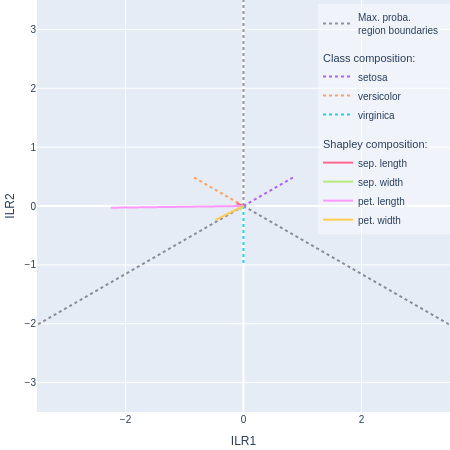
\includegraphics[width=0.8\linewidth]{figures/3classes/ilrplot.png}
    }
  \subfigure[Sum of the Shapley compositions in the ILR space from the base to the prediction]{\label{fig:3classesshapsum}
    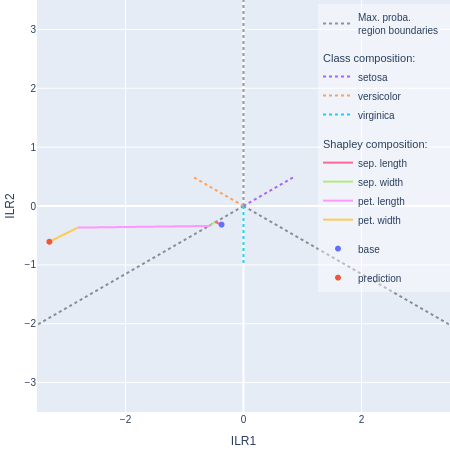
\includegraphics[width=0.8\linewidth]{figures/3classes/ilrplotsum.png}
  }
  \caption{Shapley explaination in the ILR space for the classification of an Iris instance.}
  \label{fig:3classes}
\end{figure}


\subsubsection{Four classes}

In a four classes example, the simplex is $3$-dimensional. We illustrate this with a simple digit recognition task\footnote{We use the scikit-learn's digits dataset\cite{pedregosa2011scikit}.}. It consists of classifying an $8\times8$ image as representing one of the digit among: 0, 1, 2 and 3. Since they are 64 pixels as a set of features, which would correspond to 64 Shapley composition, we reduce the number of features to 6 using a principal component analysis for better clarity. We again use a SVM classifier with an rbf kernel. The same explanation analysis as before can be applied here but within a $3$-dimensional plot as illustrated by Figure \ref{fig:4classesshapsum}. To better understand how this space is divided into four regions each representing the maximum probabity region for one class, one can think about the shape of a methane molecule. The hydrogens correspond to the vextices and the carbon to the center of a tetrahedron i.e. a $3$-dimensional simplex. The relative position of the class-compositions in the ILR space are the same as the bonds between the corbon and a hydrogen: the angles are $\approx 109.5^{\circ}$.
\begin{figure}
  \centering
  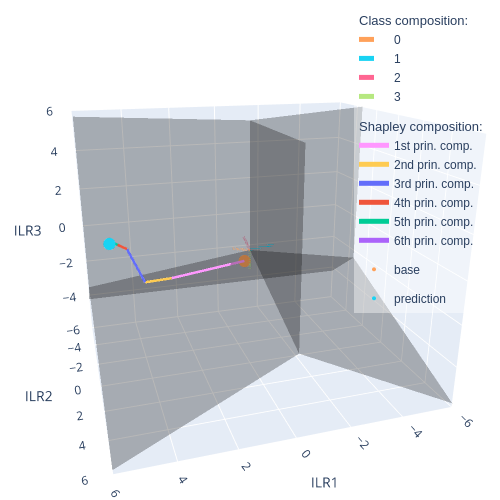
\includegraphics[width=0.9\linewidth]{figures/4classes/ilrplotsum.png}
  \caption{Shapley explaination in the $3$-dimensional ILR space for a four classes digit recognition task. The Shapley compositions are summed in the ILR space from the base distribution to the prediction.}
  \label{fig:4classesshapsum}
\end{figure}

\subsubsection{More classes}
\label{sec:moreclasses}
When there are more classes, all the dimension of the ILR space cannot be visualized at once but $2$ or $3$-dimensional subspaces can still be visualized. However, in order to choose which ILR components to visualize, one needs to understand what they refer to. For this purpose, the next section discusses the interpretation of the ILR components in more details in the context of the explanation of a classifier prediction with more than 4 classes.

\subsection{Groups of part, balances and sequential binary partition}
\ref{sec:balances}
..TODO..

\subsection{Angles, norms and projections}

Some may find the fine analysis of the features contributions in cases with more than four classes tricky. Indeed, in this case, the ILR space cannot be visualized in a $2$ or $3$-dimensional plot and as discussed in Section \ref{sec:moreclasses}, choosing which subspaces to visualize require a careful understanding of the sequential binary partition. However, as we already had the insight from the above visualization, the Shapley explaination can be summarized by sets of angles, norms and projections. Indeed the norm of a Shapley composition gives the strength of the feature's contribution in the prediction. It gives the overall contribution of the feature on the prediction, regardless of its direction. The angle between two Shapley compositions can informs if features are redundant, orthogonal or contradictory. The projection of a Shapley composition on the set of class-compositions informs in favor of, or against, which classes a feature is contributing. Appendix \ref{app:summarize}, provides some examples of summarizing a Shapley explanation using the norm of Shapley compositions, angles between them and their projection on the class-compositions.

\subsection{Histograms}

If one found hard to visualize the proposed Shapley explanation in the ILR space, the Shapley composition can be visualized as histograms like discrete probability distributions. Figure \ref{fig:histiris} shows the Shapley compositions of the Iris classification example. The more uniform the histogram is, like for the sepal length and width, the less the contribution of the feature is. In opposite, the histogram for the petal length as a high value for the versicolor class, relatively to the others, confirming the contribution of the feature toward this class.
\begin{figure}
  \centering
  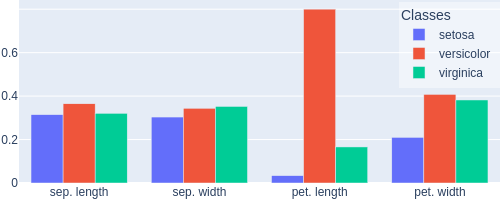
\includegraphics[width=\linewidth]{figures/3classes/histo}
  \caption{Shapley compositions visualized as histograms for the Iris classification example.}
  \label{fig:histiris}
\end{figure}
As another illustration, Figure \ref{fig:histmore} shows the Shapley compositions of the seven classes digit recognition example. Contrary to the visualization of the compositions within the ILR space as discussed in Section \ref{sec:balances}, here, one can analyses all parts of each compositions within a single plot.
\begin{figure}
  \centering
  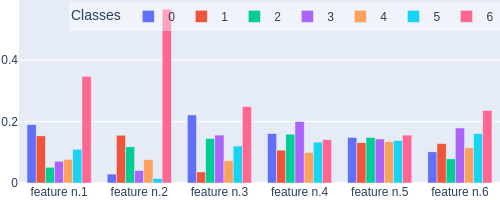
\includegraphics[width=\linewidth]{figures/moreclasses/histo}
  \caption{Shapley compositions visualized as histograms for the seven classes digit recognition example.}
  \label{fig:histiris}
\end{figure}

\subsection{About our implementation}

In this work, the estimation algorithm we used to compute the Shapley compositions is an adaptation of Algorithm 2 in \cite{vstrumbelj2014explaining}. Since the resulting Shapley compositions are approximations, the efficiency property does not necessarily hold without an adjustement. Each Shapley compositions are therefore corrected following a similar method as in the sampling approximation in the SHAP toolkit \cite{NIPS2017_7062}\footnote{\url{https://github.com/shap/shap/blob/master/shap/explainers/_sampling.py}}. See Appendix \ref{app:algo} and \ref{app:correct} for more details.

\section{Discussion and conclusion}

Compare with standard Shapley ??

We know small expé..., sounds tricky,... first step for a theoretically founded multiclass problems explanations...
...

Features INDEPENDENCE!!

Axiomatic formulation


% In the unusual situation where you want a paper to appear in the
% references without citing it in the main text, use \nocite
\nocite{langley00}

\bibliography{biblio}
\bibliographystyle{icml2024}


%%%%%%%%%%%%%%%%%%%%%%%%%%%%%%%%%%%%%%%%%%%%%%%%%%%%%%%%%%%%%%%%%%%%%%%%%%%%%%%
%%%%%%%%%%%%%%%%%%%%%%%%%%%%%%%%%%%%%%%%%%%%%%%%%%%%%%%%%%%%%%%%%%%%%%%%%%%%%%%
% APPENDIX
%%%%%%%%%%%%%%%%%%%%%%%%%%%%%%%%%%%%%%%%%%%%%%%%%%%%%%%%%%%%%%%%%%%%%%%%%%%%%%%
%%%%%%%%%%%%%%%%%%%%%%%%%%%%%%%%%%%%%%%%%%%%%%%%%%%%%%%%%%%%%%%%%%%%%%%%%%%%%%%
\newpage
\appendix
\onecolumn

\section{Linearity and efficiency of the Shapley composition}
\label{app:properties}
In this section, we show the linearity of the Shapley composition with respect to the model prediction, and the efficiency property.

\subsection{Linearity}

The Shapley composition is linear, within the Aitchison geometry of the simplex, with respect to linear combination of models' predictions.
\begin{proof}
  Let's consider the linear combination of predictions $\bm{h}(\bm{x}) = \alpha \odot \bm{f}(\bm{x}) \oplus \beta \odot \bm{g}(\bm{x})$. we want to check if:
  \begin{equation}
    \label{eq:linearsimplex}
    \bm{\phi}_{\bm{h}}(i) = \alpha \odot \bm{\phi}_{\bm{f}}(i) \oplus \beta\odot \bm{\phi}_{\bm{g}}(i).
  \end{equation}
  We have:
  \begin{equation}
    \begin{aligned}
      \mathbb{E}^{\mathcal{A}}_{\text{Pr}}[\bm{h}(\bm{x})\mid \bm{x}_S] &= \ilr^{-1} \left( \mathbb{E}_{\text{Pr}} [\ilr \left(  \alpha \odot \bm{f}(\bm{x}) \oplus \beta \odot \bm{g}(\bm{x}) \right) \mid \bm{x}_S] \right),\\
                                                                        &= \ilr^{-1} \left( \mathbb{E}_{\text{Pr}} [\alpha \ilr \left( \bm{f}(\bm{x})\right) + \beta \ilr \left( \bm{g}(\bm{x}) \right) \mid \bm{x}_S] \right),\\
                                                                        &= \ilr^{-1} \left( \alpha \mathbb{E}_{\text{Pr}} [ \ilr \left( \bm{f}(\bm{x})\right) \mid \bm{x}_S] + \beta \mathbb{E}_{\text{Pr}} [ \ilr \left( \bm{g}(\bm{x}) \right) \mid \bm{x}_S] \right),\\
                                                                        &= \alpha \odot \ilr^{-1} \left( \mathbb{E}_{\text{Pr}} [ \ilr \left( \bm{f}(\bm{x})\right) \mid \bm{x}_S] \right) \oplus \beta \odot \ilr^{-1} \left( \mathbb{E}_{\text{Pr}} [ \ilr \left( \bm{g}(\bm{x}) \right) \mid \bm{x}_S] \right),\\
                                                                        &= \alpha \odot \mathbb{E}^{\mathcal{A}}_{\text{Pr}}[\bm{f}(\bm{x})\mid \bm{x}_S] \oplus \beta \odot \mathbb{E}^{\mathcal{A}}_{\text{Pr}}[\bm{g}(\bm{x})\mid \bm{x}_S].
    \end{aligned}
  \end{equation}
  Therefore, $\bm{v}_{\bm{h},\bm{x},\text{Pr}}(\bm{X}_S) = \alpha \odot \bm{v}_{\bm{f},\bm{x},\text{Pr}}(\bm{X}_S) \oplus \beta \odot \bm{v}_{\bm{g},\bm{x},\text{Pr}}(\bm{X}_S)$, meaning that $\bm{v}$ is linear with respect to the learned function or model. The linearity of the contribution $\bm{c}$ naturally follows:
  \begin{equation}
    \begin{aligned}
      &\bm{c}_{\bm{h},\bm{x},\text{Pr}}(i,\bm{X}_S) = \bm{v}_{\bm{h},\bm{x},\text{Pr}}(\bm{X}_{S\cup\{i\}}) \ominus \bm{v}_{\bm{h},\bm{x},\text{Pr}}(\bm{X}_S),\\
      &~~~~~~~= \left( \alpha \odot \bm{v}_{\bm{f},\bm{x},\text{Pr}}(\bm{X}_{S\cup\{i\}}) \oplus \beta \odot \bm{v}_{\bm{g},\bm{x},\text{Pr}}(\bm{X}_{S\cup\{i\}}) \right) \ominus \left( \alpha \odot \bm{v}_{\bm{f},\bm{x},\text{Pr}}(\bm{X}_S) \oplus \beta \odot \bm{v}_{\bm{g},\bm{x},\text{Pr}}(\bm{X}_S) \right),\\
      &~~~~~~~= \alpha \odot \bm{v}_{\bm{f},\bm{x},\text{Pr}}(\bm{X}_{S\cup\{i\}}) \oplus \beta \odot \bm{v}_{\bm{g},\bm{x},\text{Pr}}(\bm{X}_{S\cup\{i\}}) \ominus\alpha \odot \bm{v}_{\bm{f},\bm{x},\text{Pr}}(\bm{X}_S) \ominus \beta \odot \bm{v}_{\bm{g},\bm{x},\text{Pr}}(\bm{X}_S),\\
      &~~~~~~~= \alpha \odot \left( \bm{v}_{\bm{f},\bm{x},\text{Pr}}(\bm{X}_{S\cup\{i\}}) \ominus \bm{v}_{\bm{f},\bm{x},\text{Pr}}(\bm{X}_S) \right) \oplus \beta \odot \left( \bm{v}_{\bm{g},\bm{x},\text{Pr}}(\bm{X}_{S\cup\{i\}}) \ominus \bm{v}_{\bm{g},\bm{x},\text{Pr}}(\bm{X}_S)\right),\\
      &~~~~~~~= \alpha \odot \bm{c}_{\bm{f},\bm{x},\text{Pr}}(i,\bm{X}_S) \oplus \beta \odot \bm{c}_{\bm{g},\bm{x},\text{Pr}}(i,\bm{X}_S).
    \end{aligned}
  \end{equation}
  And the linearity of the Shap composition:
  \begin{equation}
    \begin{aligned}
      \bm{\phi}_{\bm{h}}(i) &= \frac{1}{d!}  \underset{\pi}{\bigoplus}\bm{c}_{\bm{h},\bm{x},\text{Pr}}(i,\pi^{<i}_{\bm{X}}),\\
                            &= \frac{1}{d!}  \underset{\pi}{\bigoplus}\left( \alpha \odot \bm{c}_{\bm{f},\bm{x},\text{Pr}}(i,\bm{X}_S) \oplus \beta \odot \bm{c}_{\bm{g},\bm{x},\text{Pr}}(i,\bm{X}_S) \right),\\
                            &= \alpha \odot \left( \frac{1}{d!}  \underset{\pi}{\bigoplus} \bm{c}_{\bm{f},\bm{x},\text{Pr}}(i,\bm{X}_S) \right) \oplus \beta \odot \left( \frac{1}{d!} \underset{\pi}{\bigoplus}    \bm{c}_{\bm{g},\bm{x},\text{Pr}}(i,\bm{X}_S) \right),\\
                            &= \alpha \odot \bm{\phi}_{\bm{f}}(i) \oplus \beta\odot \bm{\phi}_{\bm{g}}(i).
    \end{aligned}
  \end{equation}
\end{proof}

\newpage
\subsection{Efficiency}
The efficiency property naturally holds for Shapley compositions within the Aitchison geometry.
\begin{proof}
  \begin{equation}
    \begin{aligned}
      \underset{i=1}{\overset{d}\bigoplus} \bm{\phi}_{\bm{f}}(i) & = \underset{i=1}{\overset{d}\bigoplus}\left( \frac{1}{d!} \odot \underset{\pi}{\bigoplus} \bm{c}(i,\pi_{\bm{X}}^{<i})\right),\\
                                                                 &=  \frac{1}{d!} \odot \underset{i=1}{\overset{d}\bigoplus}\left( \underset{\pi}{\bigoplus} \left( \bm{v}(\pi_{\bm{X}}^{<i+1}) \ominus \bm{v}(\pi_{\bm{X}}^{<i}) \right) \right),\\
                                                                 &=  \frac{1}{d!} \odot \underset{i=1}{\overset{d}\bigoplus}\left( \underbrace{\left(\underset{\pi}{\bigoplus} \bm{v}(\pi_{\bm{X}}^{<i+1}) \right)}_{\bm{A}_{i+1}} \ominus \underbrace{\left( \underset{\pi}{\bigoplus} \bm{v}(\pi_{\bm{X}}^{<i}) \right)}_{\bm{A}_{i}} \right),\\
                                                                 &=  \frac{1}{d!} \odot \underset{i=1}{\overset{d}\bigoplus}\left( \bm{A}_{i+1} \ominus \bm{A}_{i} \right),\\
                                                                 &=  \frac{1}{d!} \odot \left( \bm{A}_{d+1} \ominus \bm{A}_{1} \right), \text{~since we have a telescoping perturbation,}\\
                                                                 &=  \frac{1}{d!} \odot \left( \left( \underset{\pi}{\bigoplus} \bm{v}(\pi_{\bm{X}}^{<d+1}) \right) \ominus \left( \underset{\pi}{\bigoplus} \bm{v}(\pi_{\bm{X}}^{<1}) \right) \right),\\
                                                                 &=  \frac{1}{d!} \odot \left( \left( \underset{\pi}{\bigoplus} \bm{v}(\bm{X}) \right) \ominus \left( \underset{\pi}{\bigoplus} \bm{v}(\bm{X}_{\emptyset}) \right) \right),\\
                                                                 &= \bm{v}(\bm{X}) \ominus \bm{v}(\bm{X}_{\emptyset}), \text{~since $d!$ is the number of different permutation,}\\
                                                                 &= \bm{f}(\bm{x}) \ominus \mathbb{E}^{\mathcal{A}}_{\text{Pr}}[\bm{f}(\bm{X})].
    \end{aligned}
  \end{equation}
\end{proof}


\newpage
\section{Class-compositions}

A $k$-class-compositions $\bm{c}^{(k)}  \in \mathcal{S}^N$ is defined as an unit norm composition going straight to the direction of the $k$th class. This is a discrete probability distribution with maximum probability for the $k$th class and uniform values for the others. The $i$th part of the $\bm{c}^{(k)}$ is:
\begin{equation}
    c_i^{(k)} = \left\lbrace
  \begin{array}{@{}ll@{}}
    1-(N-1)p, & \text{if}\ i=k \\
    p, & \text{otherwise,}
  \end{array}\right.
\end{equation}
where $p<\frac{1}{N}$. We want the Aitchison norm of each class-composition to be one:
\begin{equation}
  \begin{aligned}
    \forall k \in \{1, \dots N \},~~~~~~\lVert \bm{c}^{(k)} \rVert_a = 1 \iff& \sqrt{\frac{1}{2N} \sum_{i=1}^N \sum_{j=1}^N \left( \log \frac{c_i^{(k)}}{c_j^{(k)}} \right)^2} = 1,\\
    \text{for clarity,}&\\\text{we drop the $(k)$ from the equations,}&\\
    \iff& \sqrt{\frac{1}{2N} \sum_{i=1}^{N}\left( \left(N-1 \right) \left( \log \frac{c_i}{p} \right)^2 + \left( \log \frac{c_i}{1-(N-1)p} \right)^2 \right)} = 1,\\
    \iff& \sqrt{\frac{1}{2N} 2(N-1) \left( \log \frac{p}{1-(N-1)p} \right)^2} =1,\\
    \text{since $p<\frac{1}{N}$ and the norm should be positive:}&\\
    \iff& \sqrt{\frac{N-1}{N}}\log \frac{1-(N-1)p}{p} =1,\\
    \iff& p = \frac{\exp \left( -\sqrt{\frac{N}{N-1}} \right)}{1+ (N-1)\exp \left( -\sqrt{\frac{N}{N-1}} \right )}.
  \end{aligned}
\end{equation}
To summarize, the $i$th part of a $k$-class-compositions $\bm{c}^{(k)} \in \mathcal{S}^N$ is given by:
\begin{equation}
    c_i^{(k)} =
  \frac{1}{1+ (N-1)\exp \left( -\sqrt{\frac{N}{N-1}} \right )} \left( \left\lbrace \begin{array}{@{}ll@{}}
     1, & \text{if}\ i=k \\
     \exp \left( -\sqrt{\frac{N}{N-1}} \right), & \text{otherwise,}
  \end{array}\right.\right).
\end{equation}
In this way, $\bm{c}^{(k)}$ is going straight to the direction of class $k$ and uniformly against all the others.


\newpage
\section{Summarizing the explanation with norms, angles and projections of Shapley compositions}
\label{app:summarize}

The Table \ref{tab:normiris} gives, for the Iris classification example of Figure \ref{fig:3classes}, the norm of each Shapley compositions, the cosine similarity between them and their projection on the set of class-compositions. Having the highest norm, this confirms that the petal length is the feature that contributed the most on the prediction. Having a close to zero inner product with the virginica class-composition, shows that this feature did not contribute to the value of the probability of of this class. It contributes neither in favor, nor in the reject of this class. Having a positive inner product with the versicolor class-composition and a negative one with the setosa class-composition, this suggest that this feature is going in favor of the class versicolor and against setosa.
\begin{table}
  \centering
  \caption{Norm of the Shapley compositions, projection on the class-compositions and cosine similarity betweeen the Shapley compositions for the Iris classification example.}
  \begin{tabular}{c|c|ccc|cccc|}
    \cline{2-9}
    & \multirow{2}{*}{norm} & \multicolumn{3}{c|}{projection on the class-compositions} & \multicolumn{4}{c|}{cosine similarity between each Shapley composition} \\
    \cline{3-9}
     & & setosa & versicolor & virginica & pet. length & pet. width & sep. length & sep. width \\
    \hline
    pet. length & 2.20  & -1.91 & 1.90 & 0.02 & 1 &$\cdot$ &$\cdot$ &$\cdot$ \\
    pet. width & 0.51 & -0.51 & 0.29 & 0.22 & 0.90 & 1 &$\cdot$ &$\cdot$ \\
    sep. length & 0.13 & -0.08 & 0.13 & -0.05 & 0.93 & 0.69 & 1 &$\cdot$ \\
    sep. width & 0.11 & -0.11 & 0.04 & 0.07 & 0.77 & 0.97 & 0.49 &1 \\
    \hline
  \end{tabular}
  \label{tab:normiris}
\end{table}

Other examples ... !!!

\newpage
\section{Estimation of the Shapley compositions}
\label{app:algo}
In this section, we present an adaptation of Algorithm 2 in \cite{vstrumbelj2014explaining} we used in this work for the estimation the Shapley compositions.

Let $d$ be the number of features. We want to optimally distribute the $m_{\text{max}}$ drawn samples over the $d$ features. Let $\hat{\bm{\phi}_i}$ be the estimation of the Shapley composition for the $i$th feature. We want to minimize the sum of squared errors: $\displaystyle\sum_{i=1}^{d} \| \hat{\bm{\phi}_i} \ominus \bm{\phi}_i \|_a^2$. Since $\hat{\bm{\phi}_i}$ is a (Aitchison) sample mean we have: $\tilde{\hat{\bm{\phi}_i}} \approx \mathcal{N}(\tilde{\bm{\phi}}_i, \frac{1}{m_i}\bm{\Sigma}^{(i)})$ and $\tilde{\hat{\bm{\phi}_i}} - \tilde{\bm{\phi}}_i \approx \mathcal{N}(\bm{0}, \frac{1}{m_i}\bm{\Sigma}^{(i)})$ where the tilde refers to the ILR transformation.
Let $\bm{\Delta_i} = \tilde{\hat{\bm{\phi}_i}} - \tilde{\bm{\phi}}_i$ and $Z_i = \| \hat{\bm{\phi}_i} \ominus \bm{\phi}_i \|_a = \| \tilde{\hat{\bm{\phi}_i}} - \tilde{\bm{\phi}}_i \|_2 = \| \bm{\Delta}_i \|_2$. The expectation of the sum of squared errors is:
\begin{equation}
  \begin{aligned}
    \mathbb{E}\left[ \sum_{i=1}^{d} Z_i^2 \right] &=   \sum_{i=1}^{d} \mathbb{E}\left[ Z_i^2 \right],\\
                                                  & =\sum_{i=1}^{d} \mathbb{E}\left[ \sum_{j=1}^{d-1}\Delta_{ij}^2 \right],\\
                                                  & =\sum_{i=1}^{d} \sum_{j=1}^{d-1} \mathbb{E}\left[\Delta_{ij}^2 \right],\\
                                                  & =\sum_{i=1}^{d} \sum_{j=1}^{d-1} \frac{1}{m_i}\Sigma_{jj}^{(i)}, \text{ since } \Delta_{ij}\approx \mathcal{Z}(0, \frac{1}{m_i}\Sigma_{jj}^{(i)}),\\
    &= \sum_{i=1}^d \frac{1}{m_i} \tr \bm{\Sigma}^{(i)}.
  \end{aligned}
\end{equation}

When a sample is drawn, the feature for which the sample will be used for improving the Shapley composition estimation is chosen to maximize $\frac{\tr \bm{\Sigma}^{(i)}}{m_i} - \frac{\tr \bm{\Sigma}^{(i)}}{m_i+1}$. Like in \cite{vstrumbelj2014explaining}, this is summarized in Algorithm \ref{alg:2}.
\begin{algorithm}
   \caption{Adaptation of the Algorithm 1 in \cite{vstrumbelj2014explaining} for approximating the Shapley composition of the $i$th feature, with model $\bm{f}$, instance $\bm{x}\in\mathcal{X}$ and $m$ drawn samples.}
   \label{alg:1}
\begin{algorithmic}
   \STATE Initialize $\bm{\phi_i}\leftarrow \ilr^{-1}(\bm{0})$
   \FOR{$1$ {\bfseries to} $m$}
   \STATE Randomly select a permutation $\pi$ of the set of indexes $\mathcal{I}$,
   \STATE Randomly select a sample $\bm{w}\in\mathcal{X}$,
   \STATE Construct two instances:
   \begin{itemize}
     \item $\bm{b}_1$: which takes the values from $\bm{x}$ for the $i$th feature and the features indexed before $i$ in the order given by $\pi$, and takes the values from $\bm{w}$ otherwise,
     \item $\bm{b}_2$: which takes the values from $\bm{x}$ the features indexed before $i$ in the order given by $\pi$, and takes the values from $\bm{w}$ otherwise.
     \end{itemize}
   \STATE $\bm{\phi}_i \leftarrow \bm{\phi}_i \oplus \bm{f}(\bm{b}_1) \ominus \bm{f}(\bm{b}_2) $
   \ENDFOR
   \STATE $\bm{\phi}_i \leftarrow \frac{\bm{\phi}_i}{m}$
\end{algorithmic}
\end{algorithm}

\begin{algorithm}
   \caption{Adaptation of the Algorithm 2 in \cite{vstrumbelj2014explaining} for approximating all the Shapley compositions by optimally distributing a maximum number of samples $m_{\text{max}}$ over the $d$ features, with model $\bm{f}$, instance $\bm{x}\in\mathcal{X}$ and $m_{\text{min}}$ the minimum number of samples each feature estimation.}
   \label{alg:2}
   \begin{algorithmic}
     \STATE Initialization: $m_{i} \leftarrow 0$, $\bm{\phi}_i \leftarrow \bm{0}$, $\forall i \in \{1, \dots d\}$,
     \WHILE{$\displaystyle \sum_{i=1}^d m_i < m_{\text{max}}$}
     \IF{$\forall i, m_i \leq m_{\text{min}}$}
     \STATE $j = \underset{i}{\text{argmax}} \left( \frac{\tr \bm{\Sigma}^{(i)}}{m_i} - \frac{\tr \bm{\Sigma}^{(i)}}{m_i+1} \right)$,
     \ELSE
     \STATE pick a $j$ such that $m_j < m_{\text{min}}$,
     \ENDIF
     \STATE $\bm{\phi}_j \leftarrow \bm{\phi}_j +$result of Algorithm \ref{alg:1} for the $j$th feature and $m=1$,
     \STATE update $\bm{\Sigma}^{(j)}$ using an incremental algorithm,
     \STATE $m_j \leftarrow m_j+1$
     \ENDWHILE
     \STATE $\bm{\phi}_i \leftarrow \frac{\bm{\phi}_i}{m_i}$, $\forall i \in \{1, \dots d\}$.
\end{algorithmic}
\end{algorithm}

\newpage
\section{Adjustement of the estimated Shapley compositions for efficiency}
\label{app:correct}

In practice, the computation of the Shapley values has an exponential time complexity and we do not have necessarily access to the true distribution of the data. The Shapley values are therefore approximated using estimation algorithms like for instance the one presented in the previous appendix. However, since the obtained values are approximations, they do not necessarily respect the desired efficiency property. This point is often overlooked in the literature. In this section we write down an adjustment strategy of the estimated Shapley compositions for them to respect the efficiency property. This is a similar strategy as in the sampling approximation of the Shapley values in the SHAP toolkit \cite{NIPS2017_7062}\footnote{\url{https://github.com/shap/shap/blob/master/shap/explainers/_sampling.py}}.

Let $\{\hat{\bm{\phi}}_i\}_{1\leq i \leq d}$ be the estimated Shapley compositions (given by the Algorithm \ref{alg:2} in our experiments). Let $\displaystyle \bm{s}_{err} = \bm{f}(\bm{x}) \ominus \bm{f}_0 \ominus \underset{i=1}{\overset{d}\bigoplus} \hat{\bm{\phi}}_i$, where is the base $\bm{f}_0$ composition, be the error composition on the pertubation of all Shapley compositions, i.e. the error making the efficiency property unfulfilled. In order to respect the efficiency property, we want this error to be the neutral element of the perturnation, i.e. the ``zero'' in the sense of the Aitchison geometry, i.e the uniform distribution. We could simply perturb each estimated Shapley compositions by $\frac{1}{d}\odot\bm{s}_{err}$ however this would move each Shapley composition by the same amount while we want to allow the compositions with a higher estimation variance (i.e. with a precision likely to be lower) to move more than the ones with a smaller variance (i.e. with a precision likely to be higher).

We therefore weight the $i$th adjustment by a scalar $w_i = w\left(\tr\left(\bm{\Sigma}^{(i)}\right)\right)$, where $w$ is an increasing function, and where $\displaystyle \sum_{i=1}^d w_i= 1$. Note that the vector of weight is actually a composition too. Similarly to the SHAP toolkit implementation, we choose $w$ as:
\begin{equation}
  w_i = w\left(\tr\left(\bm{\Sigma}^{(i)}\right)\right) = \frac{v_i}{\displaystyle 1+\sum_{j=1}^{d}v_j},\text{ where } v_i = \frac{\tr\left(\bm{\Sigma}^{(i)}\right)}{\displaystyle \epsilon \max_j \tr\left(\bm{\Sigma}^{(j)}\right)}.
\end{equation}
The $i$th estimated Shapley composition is then asjusted as follow:
\begin{equation}
  \hat{\bm{\phi}}_i \leftarrow \hat{\bm{\phi}}_i \oplus \left( w_i \odot \bm{s}_{err}\right).
\end{equation}
In this way, when $\epsilon$ goes to zero, the efficiency property is respected for the adjusted Shapley compositions and more weight is given to the adjusments of the Shapley compositions with a higher estimation variance.
%%%%%%%%%%%%%%%%%%%%%%%%%%%%%%%%%%%%%%%%%%%%%%%%%%%%%%%%%%%%%%%%%%%%%%%%%%%%%%% 
%%%%%%%%%%%%%%%%%%%%%%%%%%%%%%%%%%%%%%%%%%%%%%%%%%%%%%%%%%%%%%%%%%%%%%%%%%%%%%%


\end{document}


% This document was modified from the file originally made available by
% Pat Langley and Andrea Danyluk for ICML-2K. This version was created
% by Iain Murray in 2018, and modified by Alexandre Bouchard in
% 2019 and 2021 and by Csaba Szepesvari, Gang Niu and Sivan Sabato in 2022.
% Modified again in 2023 and 2024 by Sivan Sabato and Jonathan Scarlett.
% Previous contributors include Dan Roy, Lise Getoor and Tobias
% Scheffer, which was slightly modified from the 2010 version by
% Thorsten Joachims & Johannes Fuernkranz, slightly modified from the
% 2009 version by Kiri Wagstaff and Sam Roweis's 2008 version, which is
% slightly modified from Prasad Tadepalli's 2007 version which is a
% lightly changed version of the previous year's version by Andrew
% Moore, which was in turn edited from those of Kristian Kersting and
% Codrina Lauth. Alex Smola contributed to the algorithmic style files.

%%% Local Variables:
%%% mode: latex
%%% TeX-master: t
%%% End:
